\documentclass{article}
\usepackage[utf8]{inputenc}
\usepackage{graphicx}
\usepackage{hyperref}
\usepackage{float}
\usepackage[a4paper, total={7in, 10in}]{geometry}

\title{Relatório do Projeto SmartLock}
\author{Grupo 7}
\date{}

\begin{document}

\maketitle

\section*{Grupo 7}
\begin{itemize}
    \item Eduardo Henrique Basilio de Carvalho
    \item Guilherme Alves Sousa
    \item Leonardo Reis Domingues Paes
\end{itemize}

\section*{Repositório}
\href{https://github.com/eduardo-ufmg/EEE026_SisEmbutidos}{Repositório no Github}

\section*{Introdução}
O presente relatório aborda o desenvolvimento do projeto SmartLock, cujo objetivo principal foi conceber e implementar um sistema de controle de acesso seguro e eficiente, eliminando a necessidade de chaves mecânicas. Para tal, o sistema foi concebido para integrar múltiplas modalidades de autenticação, incluindo RFID, senhas numéricas, controle remoto via interface web e acionamento interno por chave elétrica.

\section*{Project Model Canvas}
O planejamento estratégico do projeto foi delineado por meio da ferramenta Project Model Canvas, permitindo a visualização holística dos requisitos funcionais e não funcionais, dos recursos necessários e dos desafios inerentes ao desenvolvimento. A seguir, apresenta-se a representação gráfica do Project Model Canvas adotado:

\begin{figure}[H]
    \centering
    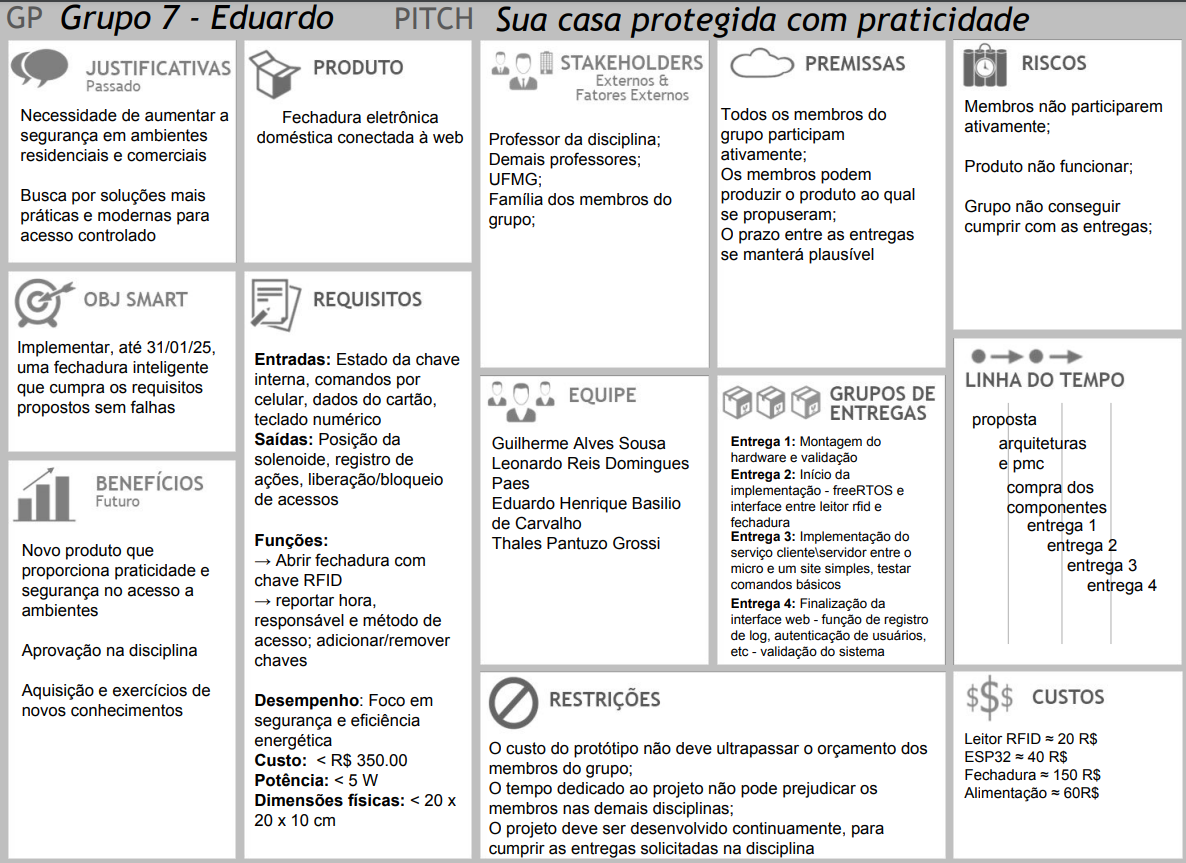
\includegraphics[width=\textwidth]{./images/pmc.png}
    \caption{Project Model Canvas}
    \label{fig:pmc}
\end{figure}

\section*{Arquitetura do Sistema}
A concepção arquitetural do sistema foi pautada na modularidade e na interoperabilidade entre os subsistemas. A seguir, são apresentadas as arquiteturas geral, de software e de hardware, detalhando os principais aspectos técnicos e organizacionais.

\subsection*{Arquitetura Geral}
A arquitetura geral do SmartLock foi projetada de forma hierárquica e distribuída, integrando sensores, atuadores e interfaces de controle por meio de um microcontrolador central. O diagrama abaixo ilustra a estrutura de alto nível do sistema:

\begin{figure}[H]
    \centering
    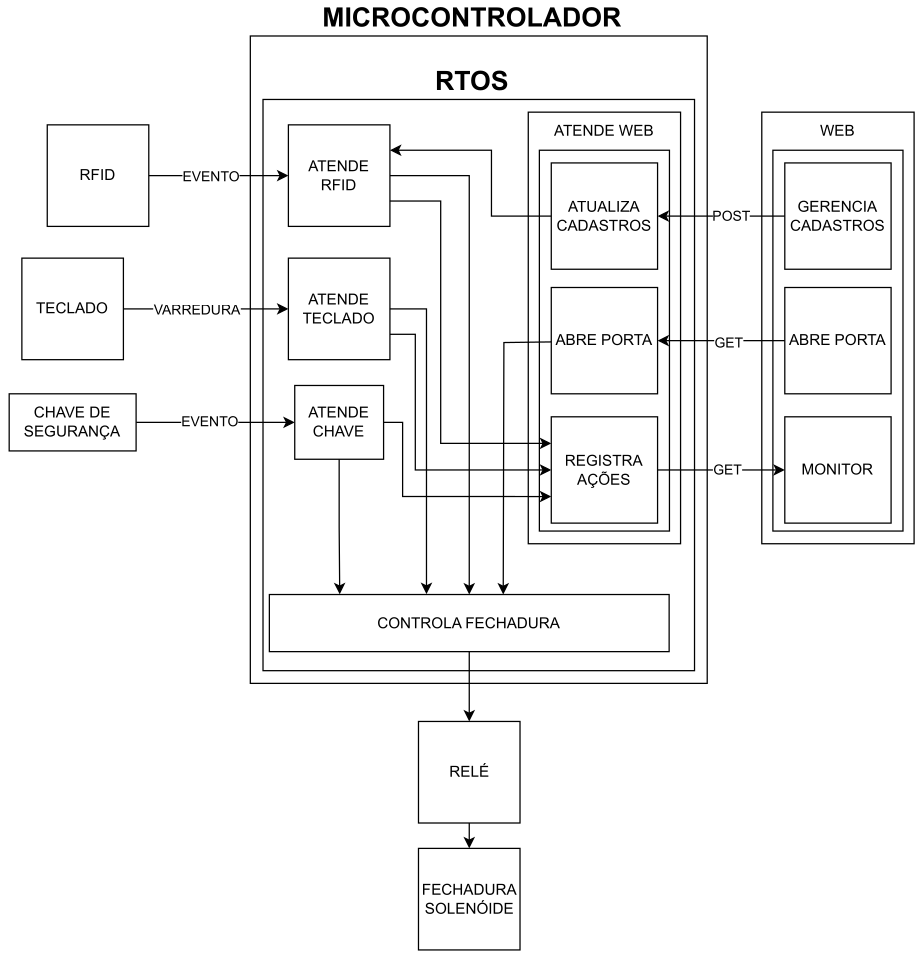
\includegraphics[width=\textwidth]{./images/arquitetura_sistema.png}
    \caption{Arquitetura de Sistema}
    \label{fig:arquitetura_sistema}
\end{figure}

\subsection*{Arquitetura de Software}
A modelagem da arquitetura de software foi baseada na separação de responsabilidades, utilizando abordagens de programação concorrente e orientada a eventos para otimizar o desempenho e a escalabilidade do sistema.

\subsection*{Arquitetura de Hardware}
A arquitetura de hardware foi estruturada para garantir compatibilidade entre os componentes e eficiência na comunicação entre dispositivos. O diagrama abaixo apresenta a interconexão dos elementos físicos e virtuais empregados no projeto:

\begin{figure}[H]
    \centering
    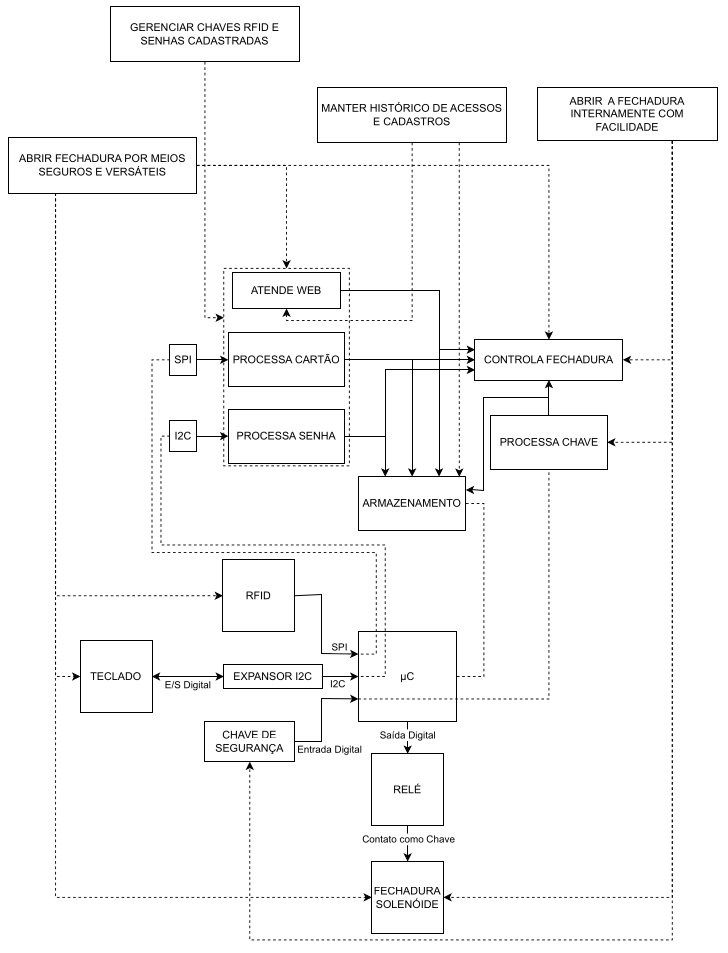
\includegraphics[width=\textwidth]{./images/arquitetura_swhw.png}
    \caption{Arquitetura de Software e Hardware}
    \label{fig:arquitetura_swhw}
\end{figure}

\section*{Desenvolvimento}
O processo de desenvolvimento contemplou a implementação de diversas funcionalidades fundamentais para a operação do SmartLock. No entanto, obstáculos técnicos e restrições temporais impediram a conclusão integral do escopo inicialmente previsto.

\subsection*{Funcionalidades Implementadas}
\begin{itemize}
    \item Autenticação por RFID
    \item Autenticação por senha numérica via teclado
    \item Controle da fechadura por relé
    \item Registro e monitoramento local de acessos
\end{itemize}

\subsection*{Funcionalidades Não Implementadas}
\begin{itemize}
    \item Interface web para gestão e monitoramento do sistema
    \item Implementação do gerenciamento remoto completo
    \item Integração com soluções avançadas de segurança
\end{itemize}

\section*{Dificuldades Encontradas}
\begin{itemize}
    \item Dificuldades na organização e comunicação entre os membros da equipe
    \item Atraso no início do desenvolvimento
\end{itemize}

\section*{Conclusão}
Embora nem todas as funcionalidades tenham sido completamente implementadas, o projeto atingiu um nível operacional que permite a autenticação e acionamento da fechadura eletrônica por múltiplos meios alternativos às chaves convencionais. Trabalhos futuros podem concentrar-se na conclusão das funcionalidades pendentes e na otimização dos componentes existentes, elevando a robustez e a confiabilidade do sistema.

\end{document}
